\documentclass[crop,tikz]{standalone}
\usetikzlibrary{shapes}
\usetikzlibrary{arrows}
\usetikzlibrary{positioning}

\begin{document}
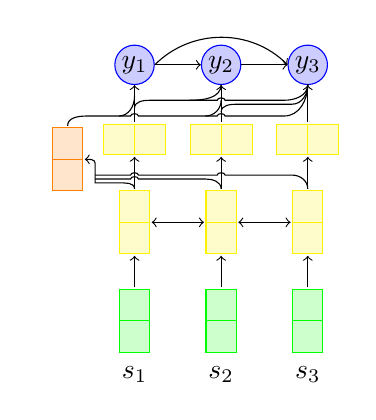
\begin{tikzpicture}[
  hid/.style 2 args={
    rectangle split,
    draw=#2,
    rectangle split parts=#1,
    fill=#2!20,
    outer sep=.25mm},
  mlp/.style 2 args={
    rectangle split,
    rectangle split horizontal,
    draw=#2,
    rectangle split parts=#1,
    fill=#2!20,
    outer sep=.25mm}
]

 % Comment out this line to remove border.
 \draw[draw=white] (-.25, 4.21) rectangle (3.8, -.4);

 \foreach \step in {1,...,3} {
   \node (i\step) at (1.1*\step, -.18) {$s_\step$};
   \node[hid={2}{green}] (e\step) at (1.1*\step, .5) {};    
 }

 \node[hid={2}{orange}] (h0) at (0.25, 2.55) {};    
  
 \foreach \step in {1,...,3} {
   \node[hid={2}{yellow}] (h\step) at (1.1 *\step, 1.75) {};    
   \draw[->] (e\step.north) -> (h\step.south);
   
   \node[mlp={2}{yellow}] (g\step) at (1.1 *\step, 2.8) {};    
   \node[circle, draw=blue, fill=blue!20,minimum size=5mm] (y\step) 
       at (1.1 *\step, 3.75) {};
   \node at (1.1 *\step, 3.75) {$y_\step$};    
   \draw[->] (g\step.north) -> (y\step.south);
   \draw[->] (h\step.north) -> (g\step.south);
 }
   
 \draw[->] (h1.north) to [out=90,in=0] (1.1 - .2, 2.25) to (0.60, 2.25)
   to [out=90,in=270] (.6, 2.35) to (.6, 2.50) to [out=90,in=0] (h0.east);
 \draw[-] (h2.north) to [out=90,in=0] (1.1 * 2 - .2, 2.30) 
     to (1.1 * 1 +.05, 2.3) to [out=90,in=90] (1.1 * 1 - .05, 2.3) 
     to (0.60, 2.30);

 \draw[-] (h3.north) to [out=90,in=0] (1.1 * 3 - .2, 2.35) 
     to (2.2 + .05, 2.35) to [out=90,in=90] (2.2 -.05, 2.35)
     to (1.1 + .05, 2.35) to [out=90,in=90] (1.1 -.05, 2.35)
     to (0.60, 2.35);

     \draw[-] (1.1,3.2) to [out=90,in=180] (1.3, 3.3) to (1.8,3.3)
        to [out=0,in=270] (2.2,3.5);
        \draw[-] (1.8,3.3) to (2.15, 3.3) to [out=90,in=90]  (2.25, 3.3)
        to (3,3.3) to [out=0,in=270] (3.3,3.5);
     \draw[-] (2.2,3.15) to [out=90,in=180] (2.4, 3.25) to (3.1,3.25)
        to [out=0,in=270] (3.3,3.5);
        \draw[-] (h0.north) to [out=90,in=180] (.5, 3.1)
        to (.9,3.1) to [out=0,in=270] (1.1,3.35);
        \draw[-] (.9,3.1) to (1.05,3.1) to [out=90,in=90] (1.15,3.1)
        to (2.0,3.1) to [out=0,in=270] (2.2,3.3);
        \draw[-] (2.0,3.1) to (2.15,3.1) to [out=90,in=90] (2.25, 3.1)
            to (3,3.1) to [out=0,in=270] (3.3, 3.5);

 % Connect document rep to labels
%% \foreach \step in {1,...,3} {
%   \draw[->] (h0.north) to [out=15,in=210]  (y\step.south);
% }
 \foreach \last/\next in {1/2, 2/3} {
   \draw[<->] (h\last.east) -> (h\next.west);
 }

 \draw[->] (y1.east) -> (y2.west);
 \draw[->] (y2.east) -> (y3.west);
 \draw [bend left=45,->] (y1.east) to (y3.west);

\end{tikzpicture}
\end{document}
